% Chapter Template
%!TEX root = ..\main.tex

\chapter{Istogrammi di gradienti orientati per classificazione di immagini} % Main chapter title
\label{cap:hog}

In questo capitolo verrà presentato il metodo di estrazione di \emph{feature} tramite istogrammi di gradienti orientati (\emph{Histogram of Oriented Gradients}, HOG). Questo metodo, introdotto per la prima volta da Dalal e Triggs \citep{Art_HOGHuman}, si basa sulla valutazione di istogrammi calcolati in base alla direzione ed alle intensità dei gradienti dell'immagine in ingresso. L'idea di base è che la forma di un oggetto possa essere rappresentata piuttosto bene mediante la distribuzione di modulo e direzione dei gradienti locali. 
\clearpage

\section{Schema generale dell'algoritmo}
Dopo aver calcolato il gradiente dell'immagine pixel per pixel, l'immagine stessa viene divisa in piccole regioni spaziali denominate "celle". Per ogni cella viene costruito un istogramma sulla base della direzione del gradiente dei  pixel in essa contenuti. Per una migliore invarianza agli effetti dovuti all'illuminazione viene effettuata una normalizzazione degli istogrammi delle celle, ottenuta sulla base di una regione spaziale di dimensione maggiore denominata "blocco". I singoli istogrammi, combinati insieme, danno origine a vettori delle \emph{feature} che vengono poi utilizzati da un classificatore, al fine di classificare l'immagine di partenza. Lo schema a blocchi del descrittore HOG è rappresentato in Figura \ref{fig:Schema_HOG}.
 \\

\tikzstyle{block} = [rectangle, draw, %fill=blue!20, 
     text width=6em, text centered, rounded corners, minimum height=3em]
\tikzstyle{line} = [draw, -latex]
%\tikzstyle{cloud} = [draw, ellipse,fill=red!20, node distance=3cm,
%    minimum height=2em]
 \begin{figure}[!ht]
    
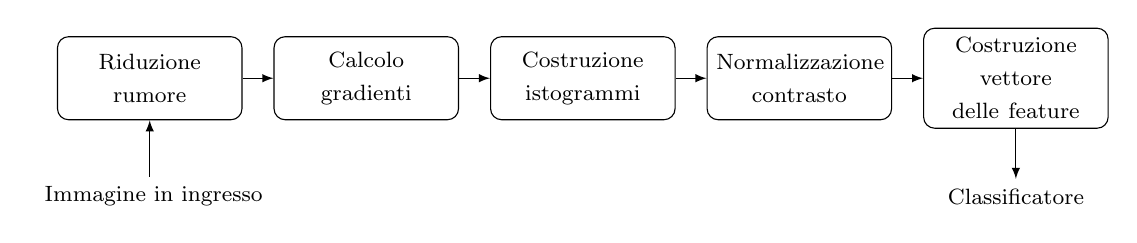
\begin{tikzpicture}[node distance = 2.75cm,]
    % Place nodes
    \node [] (input_image) {\begin{footnotesize} Immagine in ingresso \end{footnotesize}};
    \node [block, above of=input_image, node distance=1.5cm] (normalizzazione_gamma_colore) {{\footnotesize Riduzione\\ rumore}};
    \node [block, right of=normalizzazione_gamma_colore] (gradiente) {\footnotesize Calcolo gradienti};
    \node [block, right of=gradiente] (pesatura_bins) {\footnotesize Costruzione \\ istogrammi};
    \node [block, right of=pesatura_bins] (normalizzazione_blocco) {\footnotesize Normalizzazione\\ contrasto};
    \node [block, right of=normalizzazione_blocco] (features) {\footnotesize Costruzione vettore delle feature};
    \node [ below of=features,node distance=1.5cm] (classificatore) {\footnotesize Classificatore};

    % Draw edges
    \path [line] (input_image) -- (normalizzazione_gamma_colore);
    \path [line] (normalizzazione_gamma_colore) -- (gradiente);
    \path [line] (gradiente) -- (pesatura_bins);
    \path [line] (pesatura_bins) -- (normalizzazione_blocco);
    \path [line] (normalizzazione_blocco) -- (features);
    \path [line] (features) -- (classificatore);

\end{tikzpicture}
 \caption{Schema a blocchi del metodo HOG}
 \label{fig:Schema_HOG}
 \end{figure}

Di seguito verranno descritte in maniera dettagliata le singole fasi che costituiscono l'approccio HOG, evidenziando le scelte progettuali effettuate e analizzando come i diversi parametri impattino sulla prestazione.


%	SUBSECTION 1
%-----------------------------------
%\subsection{Normalizzazione Gamma/Colore}
%L'Immagine di Ingresso all'algoritmo può essere inizialmente normalizzata attraverso una correzione di gamma al fine di uniformare le diverse rappresentazioni dei pixel dell'immagine in ingresso (scala di grigio, RGB, LAB). Questa normalizzazione ha effetti limitati per quanto riguarda la performance, che invece può essere regolata variando i parametri su dimensione di celle e blocchi. Per questo  motivo abbiamo optatato per non introdurre la correzione gamma nel nostro descrittore.

%-----------------------------------
%	SUBSECTION 2
%-----------------------------------

\section{Riduzione del rumore}

%----------------------------------------------------------------------------------------
%	SECTION 2
%----------------------------------------------------------------------------------------
La strumentazione di un sensore passivo multispettrale introduce, in generale, disturbi nella misura della radianza, dovuti ad esempio ad una variazione di emittanza o illuminazione solare o, in generale, all'aleatorietà intrinseca nel processo di misura remota. Tali contributi sono indicati complessivamente con il termine di rumore. 
Questo può essere modellato come rumore additivo gaussiano\footnote{Come conseguenza del teorema centrale del limite, la distribuzione di probabilità di ogni pixel può essere modellata come gaussiana, visto l'elevato numero di contributi che concorrono alla definizione del pixel stesso.}
Per limitarne gli effetti sull'immagine di ingresso, è opportuno applicare un filtraggio per riduzione del rumore.\\

Una tipologia di filtraggio può essere ottunuta tramite la convoluzione con una gaussiana bidimensionale (Figura \ref{fig:Gaussiana3D}) il che, essendo un filtro passabasso, riduce le componenti di rumore in alta frequenza.
Lo stesso tipo di filtraggio può essere applicato anche sulle immagini in uscita dall'algoritmo HOG.\\


La funzione gaussiana $2D$ di deviazioni standard $\sigma_{x}$ $\sigma_{y}$ e coefficiente di correlazione nullo è data da:
\begin{equation}
\label{eq:Gaussiana_continua}
H_{\sigma}(x,y)= \frac{1}{\sigma_{x}\cdot \sqrt{2\pi}}\cdot e^{-\frac{x^{2}}{2(\sigma_{x})^{2}}}\cdot\frac{1}{\sigma_{y}\cdot \sqrt{2\pi}}\cdot e^{-\frac{y^{2}}{2(\sigma_{y})^{2}}}
\end{equation}

\begin{figure}[!ht]
\includegraphics[width=1\textwidth]{Gaussiana3D}
\caption{Grafico della funzione gaussiana $2D$ avente deviazioni standard $\sigma_{x}$ $\sigma_{y}$, medie nulle e coefficiente di correlazione nullo}
\label{fig:Gaussiana3D}
\end{figure}

La sua versione discreta si ottiene campionandola su una finestra quadrata di dimensioni $K \times K$ con $K> 3\cdot 2 \sqrt{\sigma}$ per rendere trascurabili gli effetti del troncamento. 
La maschera così ottenuta viene moltiplicata per $\frac{1}{c}$, dove il fattore di normalizzazione $c$ è  scelto in modo tale che 
\begin{equation}
\label{eq:normalizzazione_gaussiana}
\sum_j\sum_k g_{jk} = 1 ,
\end{equation} 
dove $g_{jk}$ è il generico elemento della gaussiana campionata.


\begin{figure}[!ht]
\centering
\subfigure[Immagine originale con rumore spazialmente uniforme]{
\includegraphics[scale=0.5]{immagine_non_filtrata}}
\hspace{3mm}
\subfigure[Risultato di filtraggio gaussiano]{
\includegraphics[scale=0.5]{immagine_filtrata}}
\caption{Riduzione del rumore nell'immagine di test tramite filtraggio gaussiano con deviazione standard pari a $\sigma = 2$ pixel}
\label{fig:immagine_rumore}
\end{figure}


\section{Calcolo dei gradienti}
Il gradiente di un'immagine misura la sua variazione direzionale di intensità.
Matematicamente, il gradiente di una funzione differenziabile di due variabili reali associa ad ogni punto del dominio un vettore 2D con componenti date dalle derivate parziali, calcolate sulle direzioni orizzontali e verticali. 
Poiché la funzione intensità di un' immagine è conosciuta solo in punti discreti, si assume che le sue derivate siano calcolate su di una funzione continua campionata nei punti dell'immagine.
\\

Dal punto di vista matematico, detta $F(x,y)$ una funzione continua e derivabile, il suo gradiente è dato da:
\begin{equation}
\label{eq:gradiente}
\nabla F=\frac{\partial F}{\partial x}\hat x + \frac{\partial F}{\partial y}\hat y
\end{equation}
dove:
\begin{itemize}
\item $\frac{\partial F}{\partial x}=G_{x}$ è la componente del gradiente calcolato lungo la direzione x;
\item $\frac{\partial F}{\partial y}=G_{y}$ è la componente del gradiente calcolato lungo la direzione y.
\end{itemize}

\begin{figure}[!ht,scale=0.8]
\centering
\subfigure[Immagine originale]{
\includegraphics[scale=0.15]{immagine_originale_primagradiente}}
\\
\subfigure[Gradiente rispetto alla direzione x]{
\includegraphics[scale=0.15]{Gradiente_rispetto_x}}
\hspace{3mm}
\subfigure[Gradiente rispetto alla direzione y]{
\includegraphics[scale=0.15]{Gradiente_rispetto_y}}
\caption{Componenti del gradienti dell'immagine di test}
\label{fig:immagine_gradienti}
\end{figure}

Nel caso di immagini bidimensionali su griglie discrete di pixel, sovente, approssimazioni di queste derivate parziali possono essere definite al variare del grado di robustezza al rumore. Il seguente schema evidenzia uno dei metodi di approssimazione più comune:
\tikzstyle{block_a} = [rectangle, draw, %fill=blue!20, 
     text width=2em, text centered, rounded corners, minimum height=3em]
\tikzstyle{block_b} = [rectangle, draw, %fill=blue!20, 
     text width=7.5em, text centered, rounded corners, minimum height=5em]
\tikzstyle{line} = [draw, -latex]
\begin{figure}[!ht]
\center
\begin{tikzpicture}[node distance = 2.5cm, every text node part/.style={align=center}]
    % Place nodes
    \node [] (input_image) at (0,0) {$I(j,k)$};
    \node [] (node1) at (1.5,0) {};
    
    \node [block_a, above right of=node1,  node distance=2cm] (gradiente_x) {$h_x$};
    \node [] () at (4.5,1.6){$G_x=I*h_x$};
    
    \node [block_a, below right of=node1, node distance=2cm] (gradiente_y) {$h_y$};
    \node [] () at (4.5,-1.7){$G_y=I*h_y$};
    %\node [] (node2) at (4,0) {};
    \node [block_b] (combinazione) at (6,0) {$G=\sqrt{G_x^2+G_y^2}$ \\ $\theta=atan(\tfrac{G_y}{G_x})$};
    \node[right of = combinazione, node distance=3cm](uscita){$\mathbf{G}(j,k)$};

    % Draw edges
    \path [line] (input_image) -- (node1);
    \path [line] (node1) |- (gradiente_x);
    \path [line] (node1) |- (gradiente_y);
    \path [line] (gradiente_x) -| (combinazione);
    \path [line] (gradiente_y) -| (combinazione);
     %\path [line] (node2) -- (combinazione);
     \path [line] (combinazione) -- (uscita);

%\begin{tikzpicture}[node distance = 3cm,]
%    % Place nodes
%    \node [] (input_image) {$I(j,k)$};
%    \node [right of=input_image, node distance=1.5cm] (node1) {};
%    \node [block, above right of=node1,  node distance=2.5cm] (gradiente_x) {Gradiente rispetto a $x$};
%     \node [block, below right of=node1, node distance=2.5cm] (gradiente_y) {Gradiente rispetto a $y$};
%     \node [below right  of=gradiente_x, node distance=2.5cm] (node2) {};
%    \node [block, right of=node2] (combinazione) {Combinazione derivate};
%    \node[right of = combinazione](uscita){$\mathbf{G}(j,k)$};
%%    \node [block, right of=pesatura_bins] (normalizzazione_blocco) {\footnotesize Normalizzazione\\ contrasto};
%%    \node [block, right of=normalizzazione_blocco] (features) {\footnotesize Costruzione vettore delle features};
%%    \node [ below of=features,node distance=1.5cm] (classificatore) {\footnotesize Classificatore};
%
%    % Draw edges
%    \path [line] (input_image) -- (node1);
%    \path [line] (node1) |- (gradiente_x);
%    \path [line] (node1) |- (gradiente_y);
%    \path [line] (gradiente_x) -| (node2);
%    \path [line] (gradiente_y) -| (node2);
%     \path [line] (node2) -- (combinazione);
%     \path [line] (combinazione) -- (uscita);
%     
%
\end{tikzpicture}

\caption{Calcolo del gradiente di un'immagine per estrazione di contorni}
\label{fig:approssimazione_gradiente}
\end{figure}

La stima di $G_{x}$ e $G_{y}$ si ottiene dall'espressione della derivata monodimensionale limitata ad un piccolo intorno (spesso solo 3 pixel).
L'approccio più semplice utilizza una risposta all'impulso monodimensionale di tipo $\left [\begin{matrix}-1 & 0 & 1\end{matrix}\right ]$.\\

Dal momento che la derivata, soprattutto quando calcolata su un intervallo così breve, è molto sensibile al rumore, si usa mediare in direzione ortogonale prima di effettuare la differenza per stabilizzarla. 
Con l'operatore di Prewitt, ad esempio, $G_{y}$ viene stimata mediante la differenza in orizzontale della media in verticale calcolata su tre punti.
Nella Tabella \ref{tab:gradiente} sono riassunti le varianti più comuni.

\begin{table}
\label{tab:gradiente}
\center
\caption{Esempi di operatori derivativi per il calcolo del gradiente}
\begin{tabular}{ccc}
 &&\\  
 & Gradiente per riga & Gradiente per colonna \\
 &&\\ 
Roberts & $\left [\begin{matrix}
0 & 0 & -1\\

0 & 1 & 0\\

0  & 0 & 0\\
\end{matrix}\right ]$& $\left[ \begin{matrix}
-1 & 0 & 0\\

0 & 1 & 0\\

0  & 0 & 0\\
\end{matrix}\right ] $ \\ 
&&\\
Prewitt
&
$\frac{1}{3}\left [
\begin{matrix}
1& 0 &-1\\
1 &0& -1\\
1 &0& -1\\
\end{matrix}\right ]$
&
$\frac{1}{3}\left [\begin{matrix}
-1 &-1& -1\\
0  &0&  0\\
1  &1&  1\\
\end{matrix}\right ]$\\
&&\\
Sobel
&
$\frac{1}{4}\left [
\begin{matrix}
-1& -2 &-1\\
0 & 0 & 0\\
1 & 2 & 1\\
\end{matrix}\right ]$
&
$\frac{1}{4}\left [\begin{matrix}
1 & 0 & -1\\
2 & 0 & -2\\
1 & 0 & -1\\
\end{matrix}\right ]$\\
&&\\
\end{tabular} 
\end{table}

Questi operatori forniscono risultati accettabili per immagini poco rumorose, infatti è opportuno che l'immagine, come introdotto precedentemente, in ingresso sia filtrata al fine di limitare gli effetti del rumore.
\\

Siano $G_{x}$ e $G_{y}$ le immagini gradiente generate da:
\begin{equation}
\label{eq:gradiente_su_x}
G_{x}(j,k)= Img(j,k) * h_{x}(j,k)
\end{equation}
\begin{equation}
\label{eq:gradiente_su_y}
G_{y}(j,k)=Img(j,k) * h_{y}(j,k)
\end{equation}
dove * rappresenta la convoluzione e dove $h_{x}$ e $h_{y}$ rappresentano rispettivamente le risposte all'impulso degli operatori descritti precedentemente.
Modulo e direzione del gradiente si ottengono, per ogni pixel dell'immagine, combinando $G_{x}$ e $G_{y}$ rispettivamente come:
\begin{equation}
\label{eq:"Forza_del_contorno"}
G(j,k)= \sqrt{(G_{x}(j,k))^2 + (G_{y}(j,k))^2}
\end{equation}
\begin{equation}
\label{eq:"Direzione_del_contorno"}
\theta(j,k)= \twopartdef{atan\left (\frac{G_{y}(j,k)}{G_{x}(j,k)}\right )}{G_y(j,k)\geq 0}{atan\left (\frac{G_{y}(j,k)}{G_{x}(j,k)}\right )+\pi}{G_y(j,k)<0}
\end{equation}
Per alcune applicazioni, il segno del gradiente, e quindi il valore di $\theta$ compreso tra $[0,2\pi]$ è rilevante per il problema di classificazione. Nella maggior parte delle applicazioni però, il segno del gradiente fornisce informazioni secondarie e irrilevanti; dunque $\theta(j,k)$ può essere calcolato nell'intervallo $[0,\pi]$.\\


\section{Costruzione degli istogrammi}
Il passo successivo al calcolo dei gradienti è quello di costruire gli istogrammi. A tale fine l'immagine di ingresso viene divisa in "celle" che possono essere di due diverse forme geometriche: rettangolari (R-HOG), di dimensioni $N\times N $ pixel, o circolari (C-HOG), di raggio $N$ pixel.\\
Per ogni cella viene creato un istogramma accumulando all'interno dei corrispondenti intervalli di quantizzazione i voti dei gradienti di ciascun pixel della cella, pesati in base al modulo del gradiente. 
Gli \emph{orientation bin} sono spaziati uniformemente nell'intervallo $[0, 2\pi]$ (gradiente con segno) o $[0, \pi]$ (gradiente senza segno).\\ 
Si considerino $n_{\theta}$ \emph{angle bin} in $[0,\pi]$ (o, come discusso in precedenza, potenzialmente, in $[0,2\pi]$).
I descrittori HOG racchiudono le statistiche locali dei gradienti (modulo e direzione) in quanto ogni pixel dà il suo voto ad uno specifico \emph{angle bin} il cui peso è proporzionale al'intensità del gradiente in quel determinato pixel. 
\\
Detto $ n_{\theta}$ il numero di \emph{angle bin} e posto ${\phi_{k}}={\frac{\pi\cdot k}{n_{\theta}}}$, con $k=0...n_{\theta}$, e dette $n_{x}$ e $n_{y}$ il numero di celle rispettivamente sulla riga e sulla colonna dell'immagine, si costruisce una matrice tridimensionale di dimensione $n_{x}\times n_{y} \times n_{\theta}$ data da:
\begin{equation}
\label{eq:euquazione_matrice_voti}
V(i,j,k)=f\left [G(i,j)\right ]\delta(\phi_{k-1} <\theta(i,j) \leq\phi_{k}), \quad \text{con} \quad k=1,\ldots,n_{\theta}
\end{equation}
dove $ \delta(x)$ restituisce $1$ quando l'argomento è vero, $0$ quando è falso e $f$ è una funzione del modulo del gradiente (lineare, radice quadrata, quadrato o una forma saturata tra quelle riportate per rappresentare la presenza o assenza di contorni).

Un'istogramma con $n_{\theta}$ canali (\emph{orientations bins}) ad esempio è costruito nel modo seguente.
\begin{itemize} 
 \item i voti di tutti i gradienti della celle che hanno un angolo compreso nell'intervallo $\left [0, \frac{\pi}{n_{\theta}}\right )$ sono accumulati nel primo canale;
 \item i voti di tutti i gradienti della celle che hanno un angolo compreso nell'intervallo $\left [\frac{\pi}{n_{\theta}}, \frac{\pi}{n_{\theta}}\cdot 2\right )$ sono accumulati nel secondo canale;
 \item i voti di tutti i gradienti della celle che hanno un angolo compreso nell'intervallo $\left [\frac{\pi}{n_{\theta}}\cdot 2,\frac{\pi}{n_{\theta}}\cdot 3\right )$ sono accumulati nel terzo canale;
 \item[] $\vdots$
 \item fino al canale $n_{\theta}$ dove sono accumulati i gradienti delle celle che hanno angolo compreso tra $\left [\frac{\pi}{n_{\theta}}\cdot {(k-1)},\frac{\pi}{n_{\theta}}\cdot k\right )$
 \end{itemize}
Formalmente, data la $c$-esima cella,l'istogramma è costruito nel seguente modo:
\begin{equation}
\label{eq:}
H(c,k)=\sum_{(i,j)\in\text{c}}V(i,j,k)=\sum_{(i,j)\in\text{c}}f[G(i,j)]\delta(\phi_{k-1}<\theta<\phi_k),  \text{con} \quad k=1,\ldots,n_\theta
\end{equation}

Il voto dato da ciascun pixel è proporzionale al'intensità del gradiente di quel punto, poiché risulta importante associare ad ogni orientazione del gradiente in un dato intervallo un voto che tenga conto dell'importanza del gradiente in un determinato pixel. 
Infatti, il gradiente calcolato attorno a un bordo risulta molto più significativo di quello calcolato in una zona uniforme dell'immagine ed è essenziale per estrarre informazioni utili ad avere una descrizione dettagliata delle strutture geometriche presenti. 

\section{Normalizzazione dei blocchi}
L'intensità del gradiente utilizzata nei descrittori HOG è sensibile ai cambiamenti locali di luminosità.
Per questo motivo è essenziale, per il raggiungimento diuna buona discriminazione fra classi nell'immagine, eseguire una normalizzazione dell'istogramma, così da introdurre una migliore invarianza a diverse condizioni di luminosità, contrasto, ombre.\\
In questa fase ogni istogramma è dunque normalizzato separatamente in base ad un fattore di normalizzazione calcolato sulla base di raggruppamenti di celle circostanti, denominati "blocchi". Ognuno di questi blocchi è composto da $M \times M$ celle.

\subsection{Schemi di normalizzazione}
Si possono valutare diversi schemi per calcolare il valore di normalizzazione. \\
Detto $\textbf{v}= \sum_{k=1}^{n_\theta} H(c,k)\hat{v}$ il vettore descrittore non ancora normalizzato e sia ${\|\textbf{v}\|}_{k}$ la sua norma $k$-esima, con $k=1,2$, si possono utilizzare i seguenti schemi come proposto da Dalal e Triggs \citep{Art_HOGHuman}:
\begin{itemize}
\item L1-Norm : $\textbf{v} \rightarrow\frac{\textbf{v}}{{\|\textbf{v}\|}_{1}+\varepsilon} $
\item L2-Norm :  $\textbf{v} \rightarrow\frac{\textbf{v}}{{\|\textbf{v}\|}_{2}^2+{\varepsilon}^2} $
\end{itemize}
dove $\varepsilon$ è una costante introdotta per evitare la divisione per zero e sufficientemente piccola da non alterare significativamente il risultato.
\\
Un altro metodo per effettuare la normalizzazione è quello proposto da Torrione e Morton \citep{Art_HOGLandmine}. \\
Detta $N$ l'insieme di celle comprese nel blocco di interesse, il valore di normalizzazione può essere calcolato come segue:
\begin{equation}
\label{eq:normalizzazione}
H(c,k)= \frac{H_{1}(c,k)}{\left ( \sum_{c_i\in N} \sqrt{\|H_{1}(c_i)\|^2_2+\varepsilon^2}\right )}
\end{equation}
dove $H_1(c,k)=\sum_{(i,j)\in c}V(i,j,k)$ e $H_1(c)$ rappresenta il vettore colonna\\
 $[H_1(c,1),\ldots, H_1(c,n_{\theta}) ]^T$.
 
 \section{Costruzione del vettore delle feature}
A questo punto si procede alla costruzione del descrittore vettoriale (\emph{feature vector}), che verrà classificato mediante un classificatore. Il descrittore avrà le stesse dimensioni dell'immagine originale con un numero di bande pari a $C + C\times B$, dove $C$ è il numero di canali dell'immagine da classificare e $B$ il numero di \emph{bin} scelto nella fase di costruzione degli istogrammi.\\
Tenendo ben presente che per immagini multispettrali l'HOG viene calcolato separatamente per ogni canale spettrale, la costruzione dei vettori delle \emph{feauture} avviene nel modo seguente: per ogni pixel vengono concatenati l'immagine originale a $C$ canali con i $C$ istogrammi, costituiti da $B$ canali ciascuno, relativi a ciascuna cella e alla banda corrispondente.\\
Matematicamente, detto $\textbf{X}_{i}$ il vettore delle \emph{feature} corrispondente all' i-esimo pixel dell'immagine:
\begin{equation}
\label{eq:feature_vector}
\textbf{X}_{i}=\left[\textbf{X}_{RGB_{i}}, \textbf{f}(\textbf{X}_{RGB_{i}})\right]
\end{equation}
con \begin{equation}
\label{eq:}
\mathbf{f}(\cdot)=(\mathbf{f}_1,\mathbf{f}_2,\ldots,\mathbf{f}_{n_\theta})
\end{equation}
dove $\textbf{f}_j$ con $j=1,2,\ldots,n_\theta$ è la componente $j$-esima dell'istogramma e $\textbf{X}_{RGB}$ è l'immagine originale.
\\
\begin{figure}[!ht]
\centering
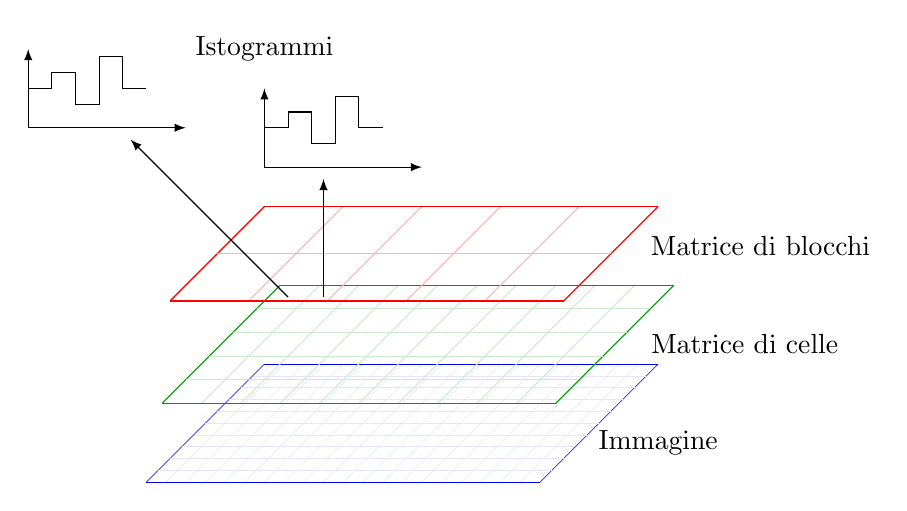
\begin{tikzpicture}
%\draw[color=gray!20] (0,0) grid (10,10);
%\draw[](0,0)--(5,0);
%\draw[](0,0)--(-1.25,-2.5);   
  
  %% griglia di pixel  
  \foreach \x in {0,0.25,0.5,...,5} \draw[color=blue!10,very thin] (\x,0)--+(-1.5,-1.5);
  \foreach \x in {0,5} \draw[color=blue,very thin] (\x,0)--+(-1.5,-1.5);
  
 \foreach \y in {0,0.15,0.3,...,1.6 } \draw[color=blue!10,very thin] (-1*\y,-\y)--+(5,0);
 \foreach \y in {0,1.5 } \draw[color=blue,very thin] (-1*\y,-\y)--+(5,0);
 
 \node[] at (5,-1){Immagine};
%  
%  %% griglia di celle
	\foreach \x in {0,0.5,1,...,5} \draw[color=green!60!black!20,thin] (\x+0.2,0+1)--+(-1.5,-1.5);
  \foreach \x in {0,5} \draw[color=green!60!black,thin] (\x+0.2,0+1)--+(-1.5,-1.5);
  
 \foreach \y in {0,0.3,0.6,...,1.6 } \draw[color=green!60!black!20,thin] (-1*\y+0.2,-\y+1)--+(5,0);
 \foreach \y in {0,1.5 } \draw[color=green!60!black,thin] (-1*\y+0.2,-\y+1)--+(5,0);
  \node[] at (6.1,0.25){Matrice di celle};
 %griglia di blocchi
	\foreach \x in {0,1,2,...,5} \draw[color=red!30,thin] (\x,0+2)--+(-1.2,-1.2);
  \foreach \x in {0,5} \draw[color=red,thin] (\x,0+2)--+(-1.2,-1.2);
  
 \foreach \y in {0,0.6,1.2 } \draw[color=red!30,thin] (-1*\y,-\y+2)--+(5,0);
 \foreach \y in {0,1.2 } \draw[color=red,thin] (-1*\y,-\y+2)--+(5,0);
  \node[] at (6.3,1.5){Matrice di blocchi};

	\draw[-latex](0.3,0.85)--+(-2,2);  	
	\draw[-latex](-3,3)--+(2,0);
	\draw[-latex](-3,3)--+(0,1);
	\draw[](-3,3.5)--+(0.3,0)--+(0.3,0.2)--+(0.6,0.2)--+(0.6,-.2)--+(0.9,-.2)--+(0.9,.4)--+(1.2,.4)--+(1.2,0)--+(1.5,0);
	
%	
%	
	\draw[-latex](0.75,0.85)--+(0,1.5);  
	\draw[-latex](0.,2.5)--+(2,0);
  	\draw[-latex](0.,2.5)--+(0,1);
  	\draw[](0,3)--+(0.3,0)--+(0.3,0.2)--+(0.6,0.2)--+(0.6,-.2)--+(0.9,-.2)--+(0.9,.4)--+(1.2,.4)--+(1.2,0)--+(1.5,0);
  	\node[] at (0,4){Istogrammi};
  \end{tikzpicture}
\caption{Schema esemplificativo della distribuzione spaziale di istogrammi, celle e blocchi}
\label{fig:HOG_Schema}
\end{figure}


%In questo capitolo verrà presentato il metodo di estrazione di \emph{feature} tramite istogrammi di gradienti orientati (\emph{Histogram of Oriented Gradients}, HOG). Questo metodo, introdotto per la prima volta da Dalal e Triggs \citep{Art_HOGHuman}, si basa sulla valutazione di istogrammi calcolati in base a direzione e intensità dei gradienti dell'immagine in ingresso. L'idea di base è che la forma di un oggetto può essere rappresentata in modo esaustivo dalla distribuzione di modulo e fase dei gradienti locali. 
%\clearpage
%
%\section{Schema generale dell'algoritmo}
%In pratica, dopo aver calcolato il gradiente dell'immagine punto per punto, essa viene divisa in piccole regioni spaziali denominate "celle". Per ogni cella viene costruito un istogramma sulla base della direzione del gradiente dei suoi pixel. Per una migliore invarianza agli effetti dovuti all'illuminazione viene effettuata una normalizzazione degli istogrammi delle celle, ottenuta sulla base di una regione spaziale di dimensione maggiore denominata "blocco". I singoli istogrammi, combinati, danno origine ai vettori delle \emph{feature} che vengono poi utilizzate da un classificatore, al fine di classificare l'immagine di partenza. Lo schema a blocchi del descrittore HOG è rappresentato in Figura \ref{fig:Schema_HOG}.
% \\
%
%\tikzstyle{block} = [rectangle, draw, %fill=blue!20, 
%     text width=6em, text centered, rounded corners, minimum height=3em]
%\tikzstyle{line} = [draw, -latex]
%%\tikzstyle{cloud} = [draw, ellipse,fill=red!20, node distance=3cm,
%%    minimum height=2em]
% \begin{figure}[!ht]
%    
%\begin{tikzpicture}[node distance = 2.75cm,]
%    % Place nodes
%    \node [] (input_image) {\begin{footnotesize} Immagine in ingresso \end{footnotesize}};
%    \node [block, above of=input_image, node distance=1.5cm] (normalizzazione_gamma_colore) {{\footnotesize Riduzione\\ rumore}};
%    \node [block, right of=normalizzazione_gamma_colore] (gradiente) {\footnotesize Calcolo gradienti};
%    \node [block, right of=gradiente] (pesatura_bins) {\footnotesize Costruzione \\ istogrammi};
%    \node [block, right of=pesatura_bins] (normalizzazione_blocco) {\footnotesize Normalizzazione\\ contrasto};
%    \node [block, right of=normalizzazione_blocco] (features) {\footnotesize Costruzione vettore delle features};
%    \node [ below of=features,node distance=1.5cm] (classificatore) {\footnotesize Classificatore};
%
%    % Draw edges
%    \path [line] (input_image) -- (normalizzazione_gamma_colore);
%    \path [line] (normalizzazione_gamma_colore) -- (gradiente);
%    \path [line] (gradiente) -- (pesatura_bins);
%    \path [line] (pesatura_bins) -- (normalizzazione_blocco);
%    \path [line] (normalizzazione_blocco) -- (features);
%    \path [line] (features) -- (classificatore);
%
%\end{tikzpicture}
% \caption{Schema a blocchi del metodo HOG}
% \label{fig:Schema_HOG}
% \end{figure}
%
%Di seguito verranno riportate in maniera dettagliata le singole fasi che lo costituiscono, evidenziando le scelte progettuali e analizzando come i diversi parametri varino la prestazione.
%
%
%%	SUBSECTION 1
%%-----------------------------------
%%\subsection{Normalizzazione Gamma/Colore}
%%L'Immagine di Ingresso all'algoritmo può essere inizialmente normalizzata attraverso una correzione di gamma al fine di uniformare le diverse rappresentazioni dei pixel dell'immagine in ingresso (scala di grigio, RGB, LAB). Questa normalizzazione ha effetti limitati per quanto riguarda la performance, che invece può essere regolata variando i parametri su dimensione di celle e blocchi. Per questo  motivo abbiamo optatato per non introdurre la correzione gamma nel nostro descrittore.
%
%%-----------------------------------
%%	SUBSECTION 2
%%-----------------------------------
%
%\section{Pulitura dal rumore}
%
%%----------------------------------------------------------------------------------------
%%	SECTION 2
%%----------------------------------------------------------------------------------------
%La strumentazione del sensore passivo multispettrale introduce, in generale, disturbi nella misura della radianza, dovuta ad esempio ad una variazione di riflettanza, emittanza o illuminazione solare indicati complessivamente con il termine di rumore. 
%Questo può essere modellato come rumore additivo gaussiano\footnote{Come conseguenza del teorema centrale del limite, la distribuzione di probabilità di ogni pixel può essere modellata come gaussiana, visto l'elevato numero di contributi di variabili che concorrono alla definizione del pixel stesso.}.
%Per limitarne gli effetti sull'immagine di ingresso, è opportuno applicare un filtraggio di pulizia dal rumore.\\
%
%La riduzione del rumore (\emph{noise cleaning}) può essere ottunuta tramite la convoluzione con una gaussiana bidimensionale (Figura \ref{fig:Gaussiana3D}) che, essendo notoriamente un passabasso, elimina o riduce le frequenze dove il contenuto spettrale di rumore è maggiore di quello delle immagini.
%Lo stesso tipo di filtraggio può essere applicato anche sulle immagini in uscita dall'algoritmo HOG.\\
%
%
%La gaussiana di varianza $\sigma_{x}$ $\sigma_{y}$ è data da:
%\begin{equation}
%\label{eq:Gaussiana_continua}
%H_{\sigma}(x,y)= \frac{1}{\sigma_{x}\cdot \sqrt{2\pi}}\cdot e^{-\frac{x^{2}}{(\sigma_{x})^{2}}}\cdot\frac{1}{\sigma_{y}\cdot \sqrt{2\pi}}\cdot e^{-\frac{y^{2}}{(\sigma_{y})^{2}}}
%\end{equation}
%
%\begin{figure}[!ht]
%\includegraphics[width=1\textwidth]{Gaussiana3D}
%\caption{Gaussiana in 3D di varianza $\sigma_{x}$ $\sigma_{y}$ e media nulla}
%\label{fig:Gaussiana3D}
%\end{figure}
%
%La sua versione discreta si ottiene campionandola su una finestra quadrata di dimensioni $K \times K$ con $K> 3\cdot 2 \sqrt{\sigma}$ per rendere trascurabili gli effetti del troncamento. 
%La maschera così ottenuta viene moltiplicata per $\frac{1}{c}$, dove il fattore di normalizzazione $c$ è  scelto in modo tale che: 
%\begin{equation}
%\label{eq:normalizzazione_gaussiana}
%\sum_j\sum_k g_{jk} = 1
%\end{equation} 
%dove $g_{jk}$ è il generico elemento della gaussiana campionata.
%
%
%\begin{figure}[!ht]
%\centering
%\subfigure[Immagine originale con rumore spazialmente uniforme]{
%\includegraphics[scale=0.5]{immagine_non_filtrata}}
%\hspace{3mm}
%\subfigure[Risultato di filtraggio gaussiano]{
%\includegraphics[scale=0.5]{immagine_filtrata}}
%\caption{Riduzione del rumore nell'immagine di test tramite filtraggio gaussiano a media nulla e varianza $\sigma = 2$ pixel}.
%\label{fig:immagine_rumore}
%\end{figure}
%
%
%\section{Calcolo dei Gradienti}
%Il gradiente di un'immagine misura la variazione direzionale di intensità della stessa.
%Matematicamente, il gradiente di una funzione a due variabili  associa ad ogni punto dell'immagine un vettore 2D con componenti date dalle derivate calcolate sulle direzioni orizzontali e verticali. 
%Poiché la funzione intensità di un' immagine è conosciuta solo in punti discreti, si assume che le sue derivate siano calcolate su di una funzione intensità continua campionata nei punti dell'immagine.
%\\
%
%Dal punto di vista matematico, detta $F(x,y)$ una funzione continua e derivabile, il suo gradiente è dato da:
%\begin{equation}
%\label{eq:gradiente}
%\nabla F=\frac{\partial F}{\partial x}\hat x + \frac{\partial F}{\partial y}\hat y
%\end{equation}
%dove:
%\begin{itemize}
%\item $\frac{\partial F}{\partial x}=G_{x}$ è il gradiente calcolato lungo la direzione x;
%\item $\frac{\partial F}{\partial y}=G_{y}$ è il gradiente calcolato lungo la direzione y.
%\end{itemize}
%
%\begin{figure}[!ht,scale=0.8]
%\centering
%\subfigure[Immagine originale]{
%\includegraphics[scale=0.15]{immagine_originale_primagradiente}}
%\\
%\subfigure[Gradiente rispetto alla direzione x]{
%\includegraphics[scale=0.15]{Gradiente_rispetto_x}}
%\hspace{3mm}
%\subfigure[Gradiente rispetto alla direzione y]{
%\includegraphics[scale=0.15]{Gradiente_rispetto_y}}
%\caption{Calcolo del gradiente per righe e per colonne dell'immagine di test}
%\label{fig:immagine_gradienti}
%\end{figure}
%
%Nel caso di immagini bidimensionali, approssimazioni di queste funzioni derivative possono essere definite al variare del grado di accuratezza. Il seguente schema evidenzia uno dei metodi di approssimazione più comune:
%\begin{figure}[!ht]
%\center
%\begin{tikzpicture}[node distance = 3cm,]
%    % Place nodes
%    \node [] (input_image) {$I(j,k)$};
%    \node [right of=input_image, node distance=1.5cm] (node1) {};
%    \node [block, above right of=node1,  node distance=2.5cm] (gradiente_x) {Gradiente rispetto a $x$};
%     \node [block, below right of=node1, node distance=2.5cm] (gradiente_y) {Gradiente rispetto a $y$};
%     \node [below right  of=gradiente_x, node distance=2.5cm] (node2) {};
%    \node [block, right of=node2] (combinazione) {Combinazione derivate};
%    \node[right of = combinazione](uscita){$\mathbf{G}(j,k)$};
%%    \node [block, right of=pesatura_bins] (normalizzazione_blocco) {\footnotesize Normalizzazione\\ contrasto};
%%    \node [block, right of=normalizzazione_blocco] (features) {\footnotesize Costruzione vettore delle features};
%%    \node [ below of=features,node distance=1.5cm] (classificatore) {\footnotesize Classificatore};
%
%    % Draw edges
%    \path [line] (input_image) -- (node1);
%    \path [line] (node1) |- (gradiente_x);
%    \path [line] (node1) |- (gradiente_y);
%    \path [line] (gradiente_x) -| (node2);
%    \path [line] (gradiente_y) -| (node2);
%     \path [line] (node2) -- (combinazione);
%     \path [line] (combinazione) -- (uscita);
%     
%
%\end{tikzpicture}
%
%\caption{Schema di approssimazione del gradiente di un'immagine}
%\label{fig:approssimazione_gradiente}
%\end{figure}
%
%La stima di $G_{x}$ e $G_{y}$ si ottiene dall'espressione della derivata monodimensionale limitata ad un piccolo intorno (spesso solo 3 punti).
%L'approccio più semplice utilizza una risposta all'impulso monodimensionale di tipo $\left [\begin{matrix}-1 & 0 & 1\end{matrix}\right ]$.\\
%
%Dal momento che la derivata, soprattutto quando calcolata su un intervallo così breve, è molto sensibile al rumore, si usa mediare in direzione ortogonale prima di effettuare la differenza per stabilizzarla. 
%Con l'operatore di Prewitt, ad esempio, $G_{y}$ viene stimata mediante la differenza in orizzontale della media in verticale calcolata su tre punti.
%Nella Tabella \ref{tab:gradiente} sono riassunti le varianti più comuni.
%
%\begin{table}
%\label{tab:gradiente}
%\center
%\caption{Operatori derivativi più usati per il calcolo del gradiente}
%\begin{tabular}{ccc}
% &&\\  
% & Gradiente per riga & Gradiente per colonna \\
% &&\\ 
%Roberts & $\left [\begin{matrix}
%0 & 0 & -1\\
%
%0 & 1 & 0\\
%
%0  & 0 & 0\\
%\end{matrix}\right ]$& $\left[ \begin{matrix}
%-1 & 0 & 0\\
%
%0 & 1 & 0\\
%
%0  & 0 & 0\\
%\end{matrix}\right ] $ \\ 
%&&\\
%Prewitt
%&
%$\frac{1}{3}\left [
%\begin{matrix}
%1& 0 &-1\\
%1 &0& -1\\
%1 &0& -1\\
%\end{matrix}\right ]$
%&
%$\frac{1}{3}\left [\begin{matrix}
%-1 &-1& -1\\
%0  &0&  0\\
%1  &1&  1\\
%\end{matrix}\right ]$\\
%&&\\
%Sobel
%&
%$\frac{1}{4}\left [
%\begin{matrix}
%-1& -2 &-1\\
%0 & 0 & 0\\
%1 & 2 & 1\\
%\end{matrix}\right ]$
%&
%$\frac{1}{4}\left [\begin{matrix}
%1 & 0 & -1\\
%2 & 0 & -2\\
%1 & 0 & -1\\
%\end{matrix}\right ]$\\
%&&\\
%\end{tabular} 
%\end{table}
%
%Questi operatori forniscono risultati accettabili solo per immagini poco rumorose, infatti è opportuno che l'immagine, come introdotto precedentemente, in ingresso sia filtrata al fine di limitare gli effetti del rumore.
%\\
%
%Siano $G_{x}$ e $G_{y}$ le immagini gradiente generate da:
%\begin{equation}
%\label{eq:gradiente_su_x}
%G_{x}(j,k)= Img(j,k) * h_{x}(j,k)
%\end{equation}
%\begin{equation}
%\label{eq:gradiente_su_y}
%G_{y}(j,k)=Img(j,k) * h_{y}(j,k)
%\end{equation}
%dove * rappresenta la convoluzione e dove $h_{x}$ e $h_{y}$ rappresentano rispettivamente la maschera per riga e per colonna scelta tra gli operatori descritti precedentemente.
%Modulo e fase del gradiente si ottengono, per ogni pixel dell'immagine, combinando $G_{x}$ e $G_{y}$ rispettivamente come:
%\begin{equation}
%\label{eq:"Forza_del_contorno"}
%G(j,k)= \sqrt{(G_{x}(j,k))^2 + (G_{y}(j,k))^2}
%\end{equation}
%\begin{equation}
%\label{eq:"Direzione_del_contorno"}
%\theta(j,k)= atan\left (\frac{G_{y}(j,k)}{G_{x}(j,k)}\right )
%\end{equation}
%Per alcune applicazioni, il segno del gradiente, e quindi il valore di $\theta$ compreso tra $[0,2\pi]$ è rilevante per il problema di classificazione. Nella maggior parte delle applicazioni però, il segno del gradiente fornisce informazioni secondarie e irrilevanti; dunque $\theta(j,k)$ può essere calcolato nell'intervallo $[0,\pi]$.\\
%
%
%\section{Costruzione degli istogrammi}
%Il passo successivo al calcolo dei gradienti è quello di costruire gli istogrammi. A tale fine l'immagine di ingresso viene divisa in "celle" che possono essere di due diverse forme geometriche: rettangolari (R-HOG), di dimensioni $N\times N $ pixel, o circolari (C-HOG), di raggio $N$ pixel.\\
%Per ogni cella viene creato un istogramma accumulando all'interno dei canali i voti dei gradienti di ciascun pixel della cella, pesati in base al modulo del gradiente. 
%Gli \emph{orientation bins} sono spaziati uniformemente nell'intervallo $[0, 2\pi]$ (gradiente con segno) o $[0, \pi]$ (gradiente senza segno).\\ 
%Si considerino $n_{\theta}$ \emph{angle bins} tra $[0,\pi]$ (o, come discusso in precedenza, potenzialmente, tra $[0,2\pi]$).
%I descrittori HOG racchiudono le statistiche locali dei gradienti (modulo e fase) in quanto ogni pixel dà il suo voto ad uno specifico \emph{angle bin} il cui peso è proporzionale alla magnitudine del gradiente in quel determinato pixel. 
%\\
%Detto $ n_{\theta}$ il numero di \emph{angle bins} e posto ${\phi_{k}}={\frac{180 \cdot k}{n_{\theta}}}$, con $k=0...n_{\theta}$, e dette $n_{x}$ e $n_{y}$ il numero di celle rispettivamente sulla riga e sulla colonna dell'immagine, si costruisce una matrice tridimensionale di dimensione $n_{x}\times n_{y} \times n_{\theta}$ data da:
%\begin{equation}
%\label{eq:euquazione_matrice_voti}
%V(i,j,k)=f\left [G(i,j)\right ]\delta(\phi_{k-1} <\theta(i,j) \leq\phi_{k}), \quad \text{con} \quad k=1,\ldots,n_{\theta}
%\end{equation}
%dove $ \delta(x)$ restituisce $1$ quando l'argomento è vero, $0$ quando è falso e $f$ è una funzione del modulo del gradiente (lineare, radice quadrata, quadrato o una forma saturata tra quelle riportate per rappresentare la presenza o assenza di contorni).
%
%Un'istogramma con $n_{\theta}$ canali (\emph{orientations bins}) ad esempio è costruito nel modo seguente.
%\begin{itemize} 
% \item i voti di tutti i gradienti della celle che hanno un angolo compreso nell'intervallo $\left [0, \frac{180}{n_{\theta}}\right )$ sono accumulati nel primo canale;
% \item i voti di tutti i gradienti della celle che hanno un angolo compreso nell'intervallo $\left [\frac{180}{n_{\theta}}, \frac{180}{n_{\theta}}\cdot 2\right )$ sono accumulati nel secondo canale;
% \item i voti di tutti i gradienti della celle che hanno un angolo compreso nell'intervallo $\left [\frac{180}{n_{\theta}}\cdot 2,\frac{180}{n_{\theta}}\cdot 3\right )$ sono accumulati nel terzo canale;
% \item[] $\vdots$
% \item fino al canale $n_{\theta}$ dove sono accumulati i gradienti delle celle che hanno angolo compreso tra $\left [\frac{180}{n_{\theta}}\cdot {k-1},\frac{180}{n_{\theta}}\cdot k\right )$
% \end{itemize}
%
%Il voto dato da ciascun pixel è proporzionale alla magnitudine del gradiente di quel punto, poiché risulta importante associare ad ogni orientazione del gradiente in un dato intervallo un voto che tenga conto dell'importanza del gradiente in un determinato pixel. 
%Infatti, il gradiente calcolato attorno a un bordo risulta molto più significativo di quello calcolato in una zona uniforme dell'immagine ed è essenziale per estrarre informazioni utili ad avere una descrizione dettagliata delle strutture geometriche presenti. 
%
%\section{Normalizzazione dei blocchi}
%La magnitudine del gradiente utilizzata nei descrittori HOG è sensibile ai cambiamenti locali in ambienti luminosi.
%Per questo motivo è essenziale per il raggiungimento di elevate prestazioni eseguire una normalizzazione dell'istogramma, così da introdurre una migliore invarianza a diverse condizioni di luminosità, contrasto, ombre.\\
%In questa fase ogni istogramma è dunque normalizzato separatamente in base ad un fattore di normalizzazione calcolato sulla base di raggruppamenti di celle circostanti, denominati "blocchi". Ognuno di questi blocchi è composto da $M \times M$ celle.
%
%\subsection{Schemi di normalizzazione dei blocchi}
%Si possono valutare diversi schemi per calcolare il valore di normalizzazione. \\
%Detto $\textbf{v}$ il vettore descrittore non ancora normalizzato e sia ${\|\textbf{v}\|}_{k}$ la sua norma $k$-esima, con $k=1,2$, si possono utilizzare i seguenti schemi come proposto da Dalal e Triggs \citep{Art_HOGHuman}:
%\begin{itemize}
%\item L1-Norm : $\textbf{v} =\frac{\textbf{v}}{{\|\textbf{v}\|}_{1}+\varepsilon} $
%\item L2-Norm :  $\textbf{v} =\frac{\textbf{v}}{{\|\textbf{v}\|}_{2}^2}+{\varepsilon}^2 $
%\end{itemize}
%dove $\varepsilon$ è una costante introdotta per evitare la divisione per zero e sufficientemente piccola da non alterare significativamente il risultato.
%\\
%Un altro metodo per effettuare la normalizzazione è quello proposto da Torrione e Morton \citep{Art_HOGLandmine}. \\
%Detta $N(c)$ l'insieme di celle comprese nel blocco di interesse, il valore di normalizzazione può essere calcolato come segue:
%\begin{equation}
%\label{eq:normalizzazione}
%H(c,k)= \frac{H_{1}(c,k)}{\left ( \sum_{c_i\in N(c)} \sqrt{\|H_{1}(c_i)\|^2_2+\varepsilon^2}\right )}
%\end{equation}
%dove $H_1(c,k)=\sum_{(i,j)\in c}V(i,j,k)$ e $H_1(c)$ rappresenta il vettore colonna\\
% $[H_1(c,1),\ldots, H_1(c,n_{\theta}) ]^T$.
% 
% \section{Costruzione del vettore delle feature}
%A questo punto si procede alla costruzione del descrittore vettoriale (\emph{feature vector}), che verrà classificato mediante un classificatore. Il descrittore avrà le stesse dimensioni dell'immagine originale con un numero di bande pari a $C + C\times B$, dove $C$ è il numero di canali dell'immagine da classificare e $B$ il numero di \emph{bins} scelto nella fase di costruzione degli istogrammi.\\
%Tenendo ben presente che per immagini multispettrali l'HOG viene calcolato separatamente per ogni canale, la costruzione dei vettori delle \emph{feauture} avviene nel modo seguente: per ogni pixel vengono concatenati l'immagine originale a $C$ canali con i $C$ istogrammi, costituiti da $B$ canali, relativi a ciascuna cella e alla banda corrispondente.\\
%Matematicamente, detto $\textbf{X}_{i}$ il vettore delle \emph{feature} corrispondente all' i-esimo pixel dell'immagine:
%\begin{equation}
%\label{eq:feature_vector}
%\textbf{X}_{i}=\left[\textbf{X}_{RGB_{i}}, \textbf{f}(\textbf{X}_{RGB_{i}})\right]
%\end{equation}
%con \begin{equation}
%\label{eq:}
%\textbf{f}(\cdot)=(\textbf{f}_1,\textbf{f}_2,\ldots,\textbf{f}_k)
%\end{equation}
%dove $\textbf{f}_k$ è la fuzione HOG calcolata sulla singola banda k-esima e $\textbf{X}_{RGB}$ è l'immagine originale.
%\\
%\begin{figure}[!ht]
%\centering
%\begin{tikzpicture}
%%\draw[color=gray!20] (0,0) grid (10,10);
%%\draw[](0,0)--(5,0);
%%\draw[](0,0)--(-1.25,-2.5);   
%  
%  %% griglia di pixel  
%  \foreach \x in {0,0.25,0.5,...,5} \draw[color=blue!10,very thin] (\x,0)--+(-1.5,-1.5);
%  \foreach \x in {0,5} \draw[color=blue,very thin] (\x,0)--+(-1.5,-1.5);
%  
% \foreach \y in {0,0.15,0.3,...,1.6 } \draw[color=blue!10,very thin] (-1*\y,-\y)--+(5,0);
% \foreach \y in {0,1.5 } \draw[color=blue,very thin] (-1*\y,-\y)--+(5,0);
% 
% \node[] at (5,-1){Immagine};
%%  
%%  %% griglia di celle
%	\foreach \x in {0,0.5,1,...,5} \draw[color=green!60!black!20,thin] (\x+0.2,0+1)--+(-1.5,-1.5);
%  \foreach \x in {0,5} \draw[color=green!60!black,thin] (\x+0.2,0+1)--+(-1.5,-1.5);
%  
% \foreach \y in {0,0.3,0.6,...,1.6 } \draw[color=green!60!black!20,thin] (-1*\y+0.2,-\y+1)--+(5,0);
% \foreach \y in {0,1.5 } \draw[color=green!60!black,thin] (-1*\y+0.2,-\y+1)--+(5,0);
%  \node[] at (6.1,0.25){Matrice di celle};
% %griglia di blocchi
%	\foreach \x in {0,1,2,...,5} \draw[color=red!30,thin] (\x,0+2)--+(-1.2,-1.2);
%  \foreach \x in {0,5} \draw[color=red,thin] (\x,0+2)--+(-1.2,-1.2);
%  
% \foreach \y in {0,0.6,1.2 } \draw[color=red!30,thin] (-1*\y,-\y+2)--+(5,0);
% \foreach \y in {0,1.2 } \draw[color=red,thin] (-1*\y,-\y+2)--+(5,0);
%  \node[] at (6.3,1.5){Matrice di blocchi};
%
%	\draw[-latex](0.3,0.85)--+(-2,2);  	
%	\draw[-latex](-3,3)--+(2,0);
%	\draw[-latex](-3,3)--+(0,1);
%	\draw[](-3,3.5)--+(0.3,0)--+(0.3,0.2)--+(0.6,0.2)--+(0.6,-.2)--+(0.9,-.2)--+(0.9,.4)--+(1.2,.4)--+(1.2,0)--+(1.5,0);
%	
%%	
%%	
%	\draw[-latex](0.75,0.85)--+(0,1.5);  
%	\draw[-latex](0.,2.5)--+(2,0);
%  	\draw[-latex](0.,2.5)--+(0,1);
%  	\draw[](0,3)--+(0.3,0)--+(0.3,0.2)--+(0.6,0.2)--+(0.6,-.2)--+(0.9,-.2)--+(0.9,.4)--+(1.2,.4)--+(1.2,0)--+(1.5,0);
%  	\node[] at (0,4){Istogrammi};
%  \end{tikzpicture}
%\caption{Schema esemplificativo della distribuzione spaziale di istogrammi, celle e blocchi}
%\label{fig:HOG_Schema}
%\end{figure}

%
%\chapter{Valutazione delle Prestazione del classificatore}
%
%\label{prestazioni_capitolo} % Change X to a consecutive number; for referencing this chapter elsewhere, use \ref{ChapterX}
%
%%\lhead{Capitolo \ref{prestazioni_capitolo}. \emph{Valutazione delle prestazioni del classificatore}} % Change X to a consecutive number; this is for the header on each page - perhaps a shortened title
%
%%----------------------------------------------------------------------------------------
%%	SECTION 1
%%----------------------------------------------------------------------------------------
%
%
%Dato un classificatore supervisionato, addestrato su un training set, è fondamentale saper valutare l'accuratezza che può essere ottenuta quando tale classificatore è applicato a valori incogniti.\\
%A tale scopo è essenziale valutare la probabilità di errore $P_e$ del classificatore, per decidere, ad esempio, se le \emph{feature} utilizzate siano sufficienti a discriminare bene le classi o se sia necessario estrarne altre (come parametri di tessitura nel caso in cui i canali spettrali non siano abbastanza discriminanti).
%\clearpage
%
%\subsection{Stima della probabilità di errore}
%In presenza di $C$ classi $\omega_1,\omega_2, \ldots, \omega_C$, detta $P_i$ la probabilità di errore \emph{a priori}, la probabilità di errore $P_e$ si può esprimere nel modo seguente:
%\begin{equation}
%\label{eq:P_e}
%P_e = P\lbrace\widehat{Y}\neq Y\rbrace= {\sum_{i=1}^C P\lbrace\widehat{Y}\neq \omega_i\vert Y = \omega_i\rbrace}P\lbrace Y =\omega_i\rbrace
%\end{equation}
%Dal momento che tale espressione è calcolabile solo in pochissimi casi semplici, per valutarla si adotta generalmente un approccio empirico, che stima la $P_e$ come la percentuale dei pixel di test classificati erroneamente.\\
%Solitamente la $P_e$ viene valutata su un insieme di campioni pre-etichettati(\emph{test set}) diverso rispetto a quello utilizzato per addestrare il classificatore(\emph{training set}). Questa tecnica, detta \emph{hold-out}, permette una misura delle prestazioni priva di \emph{bias} in quanto eseguita su istanze non utilizzate in fase di apprendimento.\\
%Per evitare il fenomeno dell'overfitting,\footnote{Si parla di overfitting quando la funzione discriminante è strettamente dipendente dai campioni di training specifici utilizzati per calcolarla ed è quindi particolarmente inefficace quando applicata a campioni incogniti} un'ipotesi fondamentale per stimare $P_e$ come frequenza relativa degli errori sul test set è che i campioni pre-etichettati siano indipendenti e identicamente distribuiti (i.i.d). Per questa ragione è buona norma prelevare i campioni di \emph{training} e di \emph{test} in regioni dell'immagine spazialmente disgiunte tra loro.\\
%E' altrettanto importante effettuare un'analisi qualitativa dell'intera mappa, mediante foto-interpretazione, come complemento alla valutazione quantitativa delle prestazioni di classificazione sui campioni di test.
%
%\subsection{Matrice di confusione e parametri di accuratezza}
%La $P_e$ fornisce una valutazione complessiva delle prestazioni del classificatore, senza però differenziare gli errori commessi in corrispondenza di classi diverse. Per una valutazione più dettagliata la matrice di confusione (confusion matrix) è la tipologia di osservazione statistica maggiormente utilizzata: il risultato della classificazione sulle aree campione viene confrontato con la verità al suolo [Congalton]. Questa è una matrice $C \times C$, il cui elemento $e_{ij}$ è il numero di pixel di test della classe $\omega_i$ che il classificatore ha assegnato alla classe $\omega_j$. Sulla diagonale $i=j$ della matrice di confusione si leggono dunque i numeri di pixel di test classificati in modo corretto. Questo tipo di analisi statistica consente non solo di quantificare il successo ottenuto dalla procedura, ma anche di focalizzare i punti critici del processo di classificazione, ovvero le classi meno distinguibili tra loro. \\
%L'accuratezza della classificazione può essere valutata con diversi parametri numerici, tra cui i più utilizzati sono:
%\begin{itemize}
%\item L' \emph{average accuracy} (AA) delle C classi è la media rispetto al numero di classi delle frazioni di pixel correttamente classificati (classe per classe), ed è data da:
%\begin{equation}
%\label{eq:AA}
%AA=\dfrac{1}{C}\sum_{i=1}^C\dfrac{e_{ij}}{\sum_{j=1}^C e_{ij}}
%\end{equation}
%\item L'\emph{overall accuracy }(OA) è la percentuale di pixel ben classificati sull'intero test set ed è data da:
%\begin{equation}
%\label{eq:OA}
%OA= \dfrac{1}{t}\sum_{i=1}^C e_{ij}
%\end{equation}
%\item Il parametro "$\kappa$", rappresenta una modifica dell' OA finalizzata a tenere conto in modo più completo della distribuzione degli errori tra le diverse classi, ed è dato da:
%\begin{equation}
%\label{eq:K}
%\kappa=\dfrac{OA-\frac{1}{t^2}\sum_{i=1}^C\sum_{j=1}^C\sum_{k=1}^C e_{ij}e_{ki}}{1-\frac{1}{t^2}\sum_{i=1}^C\sum_{j=1}^C\sum_{k=1}^C e_{ij} e_{ki}}
%\end{equation}
%dove t è il numero di pixel di test.
%\end{itemize}
